\documentclass{article}
\usepackage[margin=1in]{geometry}
\usepackage{microtype}
\usepackage{setspace}
\usepackage{amsmath}
\usepackage{parskip}
\usepackage{amssymb}
\usepackage{graphicx}

\graphicspath{{../public/}}

\parskip=4ex
\date{}
\author{}

\title{11.4 tangent Planes and Linear Approximations}

\begin{document}
  \maketitle
  \textbf{Introduction}\\
  In single-variable calculus, one of the most important concepts is linear approximation. As we zoom into toward a point on the graph of a differentiable function, said graph becomes indistinguishable from its tangent line. Hence why being able to approximate the function by a linear function is so important. This applies in three dimensions as well, where we zoom towards the point of a surface that is the graph of a differentiable function of two variables, the surface looks more like its tangent plane. Said function can be approximated by a linear function of two variables. This concept can be extended to functions of two or more variables as well.

  \textbf{Tangent Planes}\\
  Suppouse a surface $ S $ with an equation $ z=f(x,y) $, where $ f $ has continuous first partial derivatives. 

  Let $ P(x_{0},y_{0},z_{0})$ be a point on $ S $. Then we have two curves, $ C_{1} ~\&~ C_{2}$ obtained from intersecting the verticle planes $ y=y_{0} ~\&~ x=x_{0}   $. The point $ P $ lies on both curves $ C_{1} ~\&~ C_{2}$. $ T_{1} ~\&~ T_{2}$ are the tangent lines to its curves $ C_{1} ~\&~ C_{2}$ at the point $ P $.  

  Then the tangent plane to the surface $ S $ at the point $ P $ is the plane containing both tangent lines $ T_{1} ~\&~ T_{2}$.  
  \begin{center}
    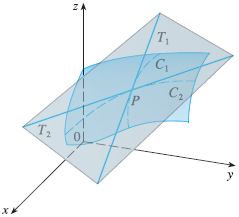
\includegraphics[width=4cm]{11_4_1}
  \end{center}

  Recall the equation for a plane passing through the point $ P(x_{0},y_{0} ,z_{0})$
  \[
    A(x-x_{0} )+B(y-y_{0} )+C(z-z_{0} )=0
  \]
  We can achieve an equation for finding $ z -z_{0} $ by dividing by $ C $
  \[
    \begin{gathered}
    \frac{A(x-x_{0} )+B(y-y_{0} )+C(z-z_{0} )}{C}=\frac{0}{C}\\
    ~\\
    z-z_{0}=-\frac{A}{C}(x-x_0)-\frac{B}{C}(y-y_{0} )\\
    \end{gathered}
  \]
  Further on we can let $ a=-\frac{A}{C} ~\&~ b=-\frac{B}{C}$ to get
  \[
    z-z_{0} =a(x-x_{0} )+b(y-y_{0} )
  \]

  Now we can also say that the intersection with the plane $ y=y_{0}$ must be the tangent line $ T_{1}$
  \[
    \begin{gathered}
    z-z_{0}=a(x-x_{0})+b(y_{0} -y_{0} ) \to 
    z-z_{0}=a(x-x_{0} ) 
    \end{gathered}
  \]
  
  This can be recognized as a point slope form equation with slope $ a $. From Section 11.3, we know that the slope of the tangent $ T_{1}  $ is $ f_{x} (x_{0},y_{0})$. 

  The same can also be done to achieve a point slope form equation with $ b $ as the slope. That being said the intersection with the plane $ x=x_{0}  $ must be the tangent line $ T_{2} $. 
  \[
    \begin{gathered}
    z-z_{0}=a(x_{0} -x_{0})+b(y -y_{0} ) \to 
    z-z_{0}=b(y-y_{0} ) 
    \end{gathered}
  \]
  Based on our previous statement for the slope of the $ T_{1}  $, we can say that the slope of the tangent $ T_{2}  $ is $ f_{y}(x_{0},y_{0}  )  $  

  Now suppouse that $ f $ has continuous partial derivatives. The equation of the tangent plane to the surface $ z=f(x,y) $ at the point $ P(x_{0},y_{0},z_{0}   ) $ is
  \[
    z-z_{0}=f_{x}(x_{0},y_{0}  )(x-x_{0})+f_{y}(x_{0},y_{0}  )(y-y_{0} )   
  \]

  \textbf{Ex 1}\\
  Find the tangent plane to the elliptic paraboloid $ z=2x^{2}+y^{2}   $ at the point $ (1,1,3) $
  \[
    \begin{gathered}
    f(x,y) = 2x^{2}+y^{2}\\
    ~\\
    f_{x}(x,y)=4x \qquad f_{y}(x,y)=2y\\
    f_{x}(1,1)=4 \qquad f_{y}(1,1)=2\\
    ~\\
     z-z_{0}=f_{x}(x_{0},y_{0}  )(x-x_{0})+f_{y}(x_{0},y_{0}  )(y-y_{0} )\\
     ~\\
     z-3=4(x-1)+2(y-1)\to \boxed{4x+2y-3}   
    \end{gathered}
  \]

  \textbf{Linear Approximations}\\
  In Example 1, we found an equation of the tangent plane to the graph of the function $ f(x,y)=2x^{2}+y^{2}   $ at the point $ (1,1,3) $ is $ z=4x+2y-3 $. Therefore the linear function of two variables
  \[
    L(x,y)=4x+2y-3
  \]
  is a good approximation to $ f(x,y) $ when $ x,y $ is near $ (1,1) $. The function $ L $ is called the linearization of $ f $ at $ (1,1) $ and the approximation $ f(x,y) \approx 4x+2y-3 $ is known as the linear approximation or tangent plane approximation of $ f $ at $ (1,1) $.

  To exemplify, we can approximate $ f(1.1,0.95)$ by plugging in the point $ (1.1,0.95) $ into the $ L(x,y) $ 
  \[
    f(1.1,0.95)=3.3225
    f(1.1,0.95) \approx 4(1.1) + 2(0.95)-3=3.3
  \]
  
  As shown $ L(x,y) $ is fairly close, but if we were to use a point farther away from $ (1,1) $, the accuracy falls off.
  \[
    f(2,3)=17 \qquad L(2,3)=11
  \]
  
  Knowing the equation of a tangent plane to the graph of a function $ f $ of two variables at the point $ a,b,f(a,b)$, we can rewrite the equation like so  
  \[
    \begin{gathered}
     z-z_{0}=f_{x}(a,b  )(x-a)+f_{y}(a,b)(y-b)\\
     ~\\
     z=z_{0}+f_{x}(a,b  )(x-a)+f_{y}(a,b  )(y-b)\\
     ~\\
     z=f(a,b) +f_{x}(a,b  )(x-a)+f_{y}(a,b  )(y-b)\\
    \end{gathered}
  \]

  If $ f_{x} ~\&~ f_{y}$ are both continuous, the linear function whpse graph is this tangent plane
  \[
    L(x,y)=f(a,b)+f_{x}(a,b)(x-a)+f_{y}(a,b)(y-b)  
  \]
  is the linearization of $ f $ at $ (a,b) $ and the approximation
  \[
  f(x,y)\approx f(a,b)+f_{x}(a,b)(x-a)+f_{y}(a,b)(y-b)
  \]
  is called the linear approximation or the tangent plane of $ f $ at $ (a,b) $.

  \textbf{Theorem}\\
  If the partial derivatives $ f_{x} ~\&~ f_{y} $ exist near $ (a,b) $ and are continuous at $ (a,b) $, then $ f $ is differentiable at $ (a,b) $.     

  \textbf{Ex 2}\\
  Show that $ f(x,y)=xe^{xy}  $ is differentiable at $ (1,0) $ and find its linearization there. Then $ f $ is differentiable at $ (1.1,-0.1)$.
  \[
    \begin{gathered}
      f_{x}(x,y)=e^{xy}+xye^{xy} \qquad f_{y}(x,y)=x^{2}e^{xy}\\
      f_{x}(1,0)=1 \qquad f_{y}(1,0) = 1\\
      ~\\
      f_{x} ~\&~ f_{y}=\text{continuous functions so} f \text{is differntiable.}\\
      ~\\
      L(x,y)=f(1,0)+f_{x}(1,0)(x-1)+f_{y}(1,0)(y-0)\\
      1+1(x-1) + 1(y-0)=x+y\\
      ~\\
      \boxed{xe^{xy}\approx x+y}\\
    f(1.1,-0.1) \approx 1.1 - 0.1 = \boxed{1} 
    \end{gathered}
  \]

  \textbf{Differentials}\\
  For a differentiable single variable function, $ y=f(x) $, the differential $ dx $ is defined to be an independent variable. Meaning that $ dx = \mathbb{R}$. So the differential of $ y $ can be defined as
  \[
    dy=f'(x)~dx
  \]
  
  Now in the case of double variable differentiable functions, $ z=f(x,y) $, the differentials $ dx ~\&~ dy $ are defined as independent variables also. So the differential $ dz $, which is also known as the total differential, is defined like so
  \[
    dz=f_{x}(x,y)~dx+f_{y}(x,y)~dy=\frac{\alpha z}{\alpha x}dx+\frac{\alpha z}{\alpha y}~dy   
  \]

  \textbf{Ex 3A}\\
  If $ z=f(x,y)=x^{2}+3xy-y^{2}$, find the differential $ dz $.
  \[
    \begin{gathered}
      dz=f_{x}(a,b)~dx+f_{y}(a,b)~dx\\
      ~\\
      \boxed{dz=(2x+3y)~dx+(3x-2y)~dy}
    \end{gathered}
  \]

  \textbf{Ex 3B}\\
  If $ x $ changes from to $ 2 \to 2.05$ and $ y $ changes from $ 3\to 2.96 $, compare the values of $ \Delta z  ~\&~ dz$.
  \[
    \begin{gathered}
    x=2,~y=3 \qquad dx=\Delta x =0.05,~dy=\Delta y =-0.04\\
    ~\\
    dz=[2(2)+3(y)]~\Delta x + [3(2)-2(3)]\Delta y=\boxed{0.65}
    \end{gathered}
  \]

  \textbf{Ex 4}\\
  The base radius and height of a right circular cone are measured as $ 10cm ~\&~ 25cm $, respectively with a $ 0.1cm$ margin of error in each measurements. Use differentials to estimate the maximum error in the calculated volume of the cone.
  \[
    \begin{gathered}
    V=\frac{\pi r^{2} h}{3}\\
    ~\\
    dV=f_{r}(a,b)~dr+f_{h}(a,b)~dy\\
    ~\\
    dV=\frac{2\pi rh}{3}~dr+\frac{\pi r^{2} }{3}~dy\\
    ~\\
    | \Delta r | \le 0.1 \qquad \Delta h | \le 0.1\\
    ~\\
    dr=0.1,~dh=0.1\\
    ~\\
    dV=0.1(\frac{500\pi}{3}) +(0.1)\frac{100\pi}{3}=\boxed{20\pi}\\
    ~\\
    \text{The maximum error in the calculated volumne is } 20\pi cm^{3} \approx 63 cm^{3} 
    \end{gathered}
  \]
\end{document}
